\documentclass[nooutcomes]{ximera}
%% handout
%% space
%% newpage
%% numbers
%% nooutcomes


\newcommand{\RR}{\mathbb R}
\renewcommand{\d}{\,d}
\newcommand{\dd}[2][]{\frac{d #1}{d #2}}
\renewcommand{\l}{\ell}
\newcommand{\ddx}{\frac{d}{dx}}
\newcommand{\dfn}{\textbf}
\newcommand{\eval}[1]{\bigg[ #1 \bigg]}

\usepackage{multicol}

\renewenvironment{freeResponse}{
\ifhandout\setbox0\vbox\bgroup\else
\begin{trivlist}\item[\hskip \labelsep\bfseries Solution:\hspace{2ex}]
\fi}
{\ifhandout\egroup\else
\end{trivlist}
\fi} %% we can turn off input when making a master document

\title{Recitation \#4 - 2.3:  Limit Laws (Solutions)}  

\begin{document}
\begin{abstract}		\end{abstract}
\maketitle

\section*{Warm up:} 
Below is a table listing all of the Limit Laws, followed by an argument of what the limit of $ \frac{5x^3 - 4 \sqrt{x}}{\sqrt{x^5 - 87}}  $ as $x$ approaches 3 must be.  State which limit law is used to justify each step.

	\begin{image}
	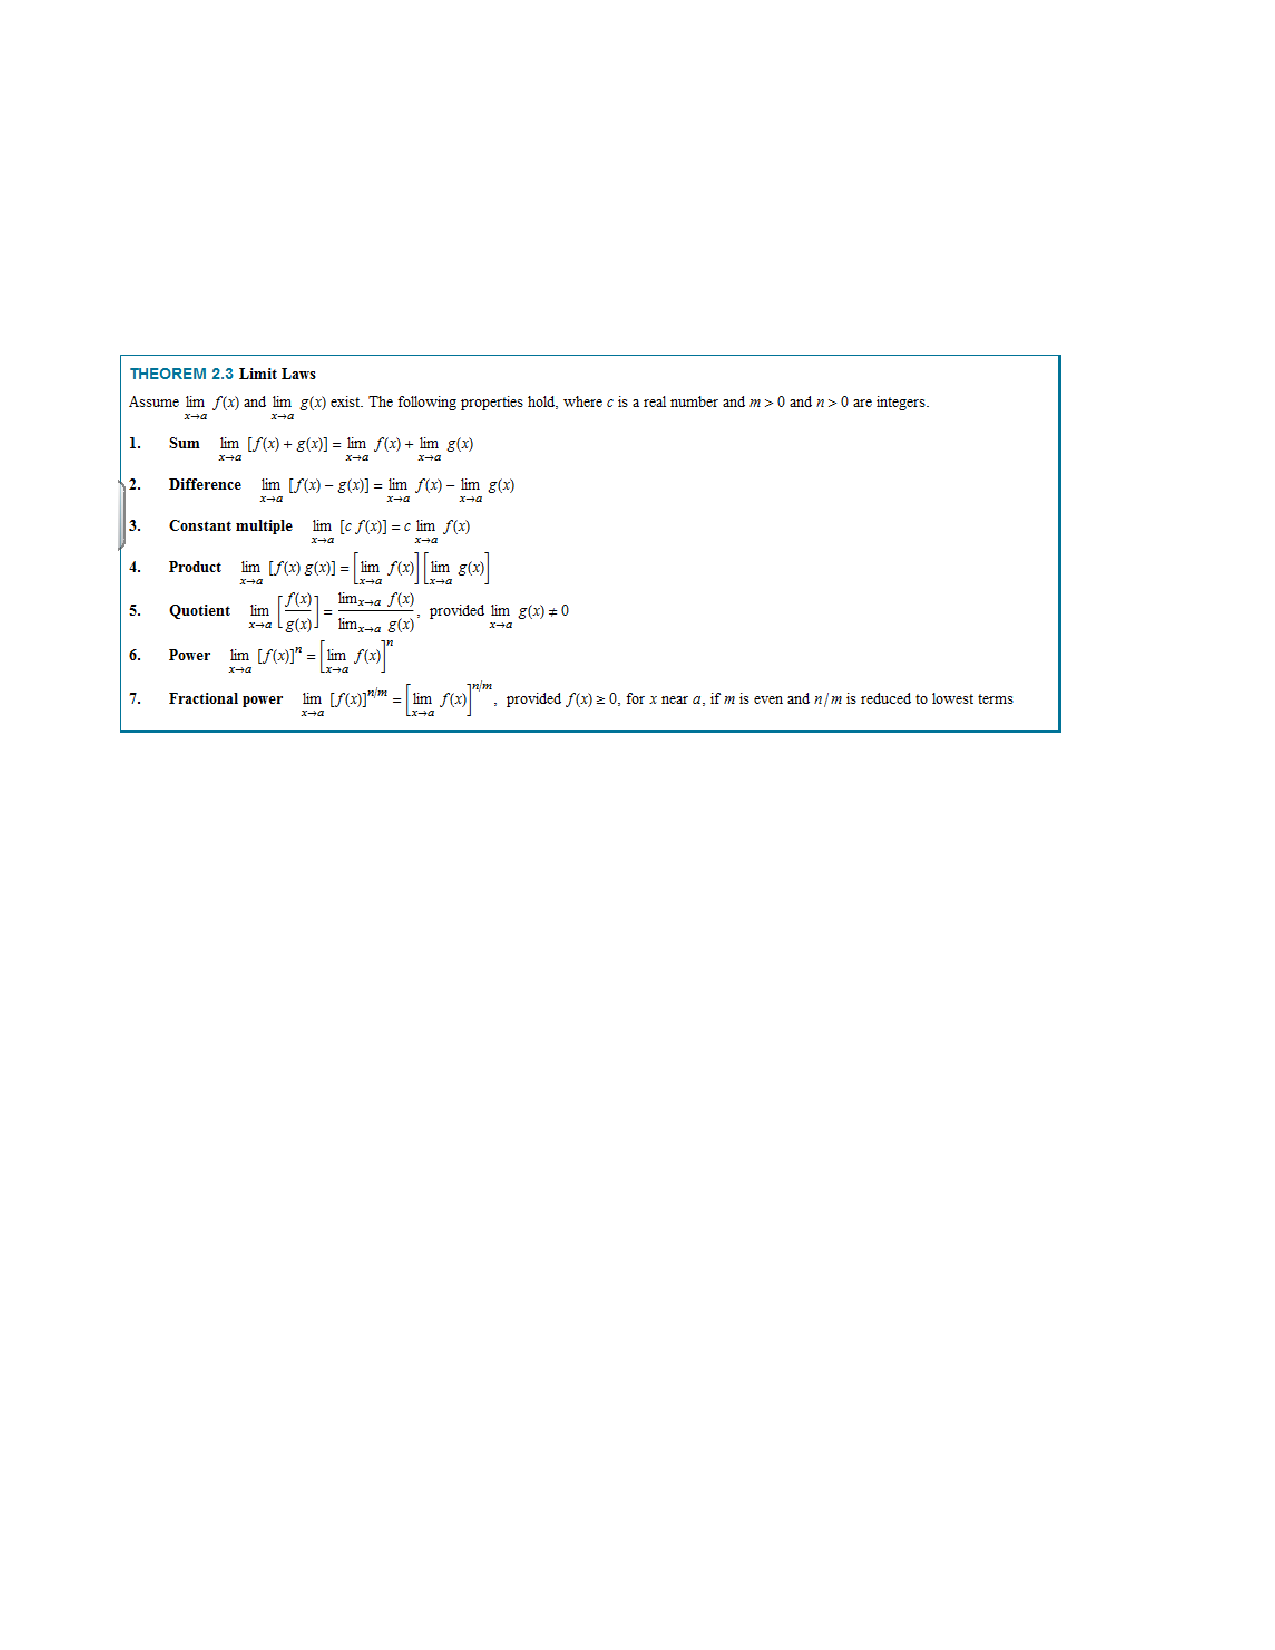
\includegraphics[trim= 250 440 300 175]{Figure1.pdf}
	\end{image}

	\begin{image}
	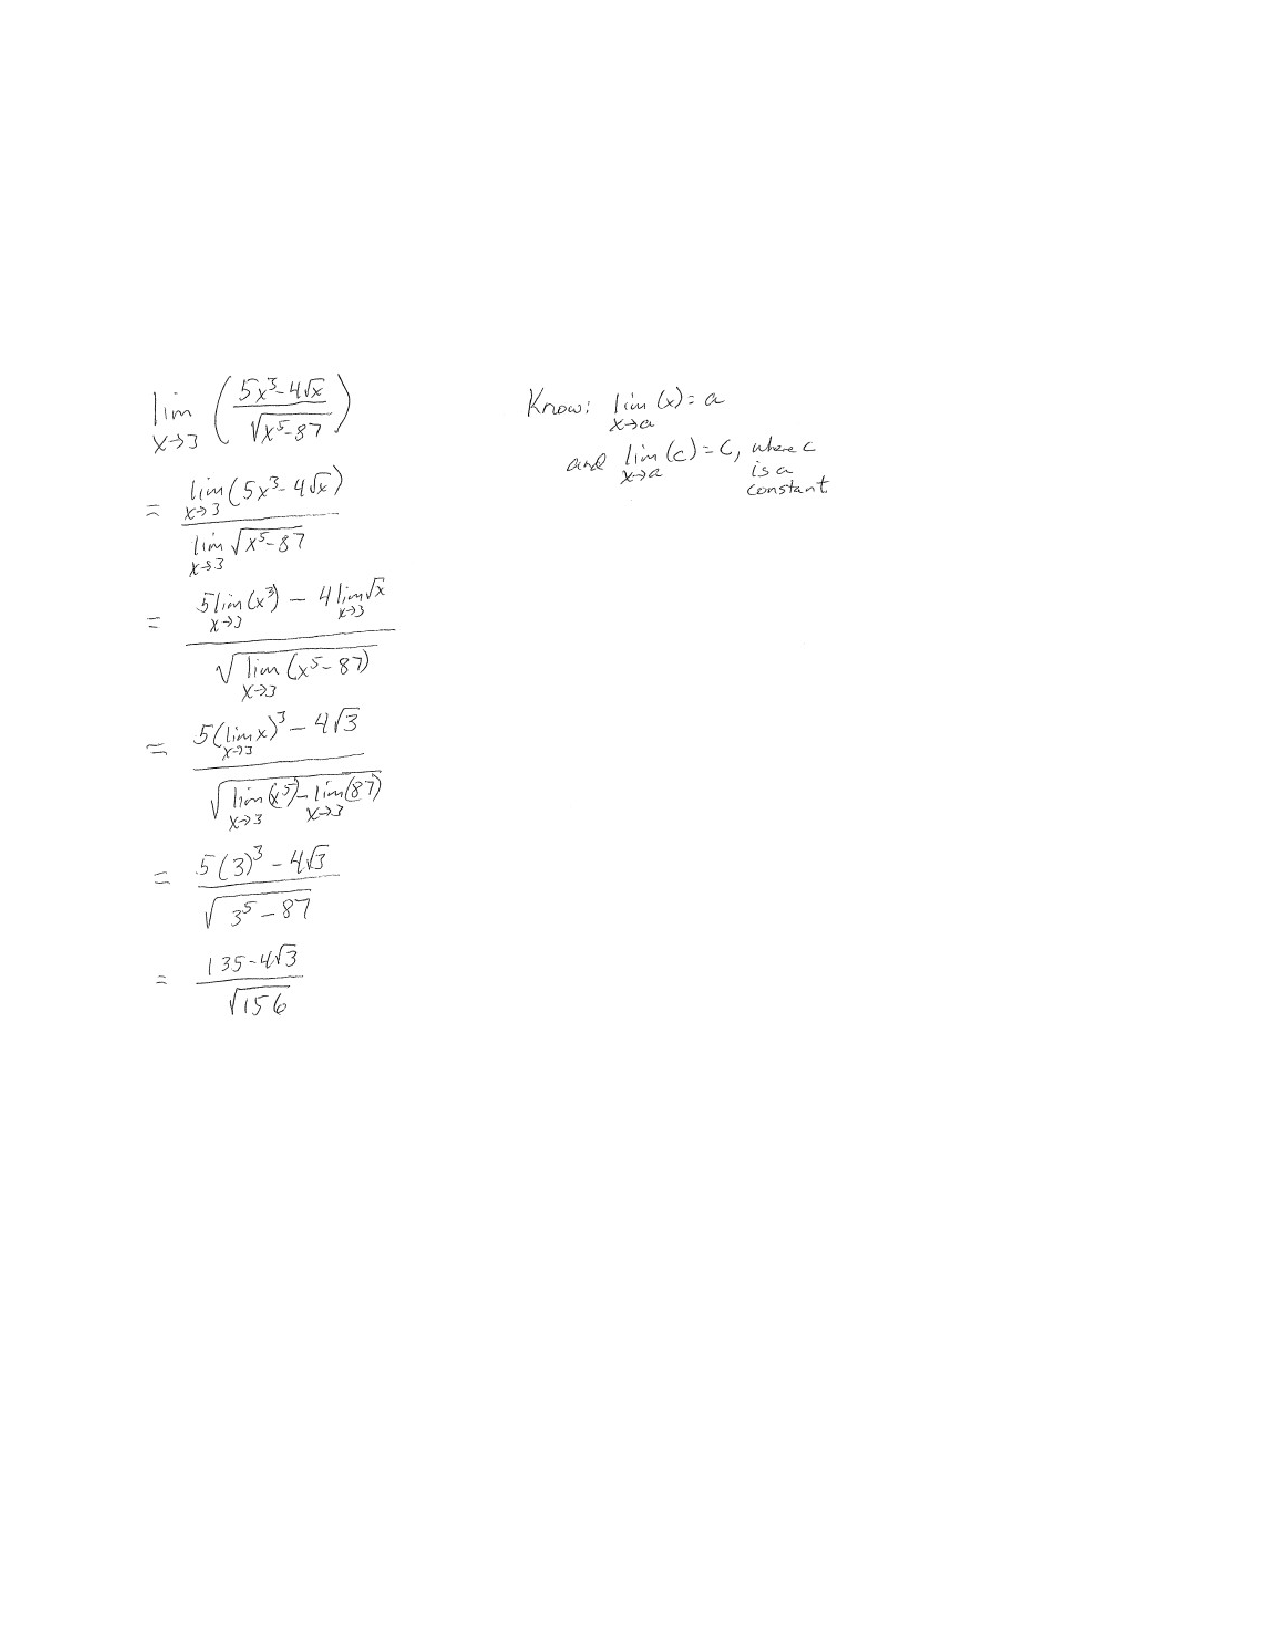
\includegraphics[trim= 150 440 300 185]{Figure2.pdf}
	\end{image}
\newpage
	\begin{freeResponse}
	Step 1:  Limit law 5.
		
	Step 2:  Limit laws 2 and 3 in the numerator, limit law 7 in the denominator.
		
	Step 3:  In the numerator both limit law 6 as well as the fact that $\lim_{x \to a}x = a$ are used.  Limit law 2 is used in the denominator.
		
	Step 4:  $\lim_{x \to a}x = a$ is used in the numerator.  This same fact, in conjunction with limit law 6, is used in the denominator.
		
	Step 5:  This step is just arithmetic.
	\end{freeResponse}
	
	

\section*{Group work:}

\begin{problem}
Evaluate the following limits algebraically using the limit laws.  
	
	\begin{enumerate}
			
	\item $ \lim_{x \to 6} \frac{4x^2 - 144}{x-6}  $
	\begin{freeResponse}
	$ \lim_{x \to 6} \frac{4x^2 - 144}{x-6} = \lim_{x \to 6} \frac{4(x-6)(x+6)}{x-6} = \lim_{x \to 6} 4(x+6) = 4(12) = 48  $
	\end{freeResponse}
	
	
			
	\item  $ \lim_{x \to 6} \frac{x-6}{\sqrt{2x-8} - 2}  $
	\begin{freeResponse}
	$ \lim_{x \to 6} \frac{x-6}{\sqrt{2x-8} - 2} \cdot \frac{\sqrt{2x-8} + 2}{\sqrt{2x-8}+2} = \lim_{x \to 6} \frac{(x-6)(\sqrt{2x-8} + 2)}{2x - 8 - 4} = \lim_{x \to 6} \frac{(x-6)(\sqrt{2x-8} + 2)}{2(x-6)} = \lim_{x \to 6} \frac{\sqrt{2x-8}+2}{2} = \frac{\sqrt{12-8}+2}{2} = \frac{4}{2} = 2 $
			
	\end{freeResponse}
	
	
			
	\item  $ \lim_{x \to 2} \frac{(3x-2)^2 - 16}{x-2}  $
	\begin{freeResponse}
	$\lim_{x \to 2} \frac{(3x-2)^2-16}{x-2}=\lim_{x \to 2} \frac{((3x-2)-4)((3x-2)+4)}{x-2}= \lim_{x \to 2} \frac{(3x-6)(3x+2)}{x-2} $
			
	$\lim_{x \to 2} \frac{3(x-2)(3x+2)}{x-2} = \lim_{x \to 2} 3(3x+2) = 3(6+2) = 24   $
	\end{freeResponse}
	
	
			
	\item  $ \lim_{x \to 1} \frac{\sqrt{5x-2} - \sqrt{3}}{x-1} $
	\begin{freeResponse}
	$\lim_{x \to 1} \frac{\sqrt{5x-2} - \sqrt{3}}{x-1} \cdot \frac{\sqrt{5x-2} + \sqrt{3}}{\sqrt{5x-2} + \sqrt{3}} = \lim_{x \to 1} \frac{(5x-2)-3}{(x-1)(\sqrt{5x-2} + \sqrt{3})}$
			
	$= \lim_{x \to 1} \frac{5(x-1)}{(x-1)(\sqrt{5x-2} + \sqrt{3})} = \lim_{x \to 1} \frac{5}{\sqrt{5x-2} + \sqrt{3}} =   \frac{5}{\sqrt{5(1)-2} + \sqrt{3}} = \frac{5}{2 \sqrt{3}} $
	\end{freeResponse}
	\end{enumerate}
\end{problem}
	
	
	
	
			
			
			
\begin{problem}
Suppose
	$f(x) =   \left\{ \begin{array}{lr}
	x^2 - ax 	&	\text{if } x < 3	\\
	a2^x + 7 + a	&	\text{if } x > 3	\end{array} \right.  $
	
	Find $a$ so that $ \lim_{x \to 3} f(x)  $ exists.
	\begin{freeResponse}
	 We need to find $a$ so that $\lim_{x \to 3^-} f(x) = \lim_{x \to 3^+} f(x) $.  
	
	\begin{itemize}
	
	\item  $\lim_{x \to 3^-} f(x) = \lim_{x \to 3^-} (x^2 - ax) = 9 - 3a $.
	
	\item  $\lim_{x \to 3^+} f(x) = \lim_{x \to 3^+} a2^x + 7 + a = a2^3 + 7 + a = 9a + 7 $
	
	\end{itemize}
	
	So we want $a$ to be such that:
	
	$ 9-3a = 9a+7 $  
	
	$12a = 2 $
	
	$a = \frac{1}{6}   $
	\end{freeResponse}
\end{problem}
	
	
	
	
	
	
	
	
	
	
\begin{problem}
Sketch the graph of a function with the given properties.  You need not find a formula for the function:
	
	$ f(3) = -2, \, f(-2) = 3, \, f(5) = 6, \, \lim_{x \to 5^-} f(x) = -1, \, \lim_{x \to 5^+} f(x) = 4, \, \lim_{x \to 3} f(x) = 7  $
	
	$ \lim_{x \to -2^-} f(x) = 3, \, \lim_{x \to -2^+} f(x) = 0, \, \lim_{x \to 1^+} f(x) = 5  $
	
	\begin{freeResponse}
	There exist infinitely many functions whose graph satisfies the conditions above, but one such graph is the following:
	
\newpage
	
		\begin{image}
		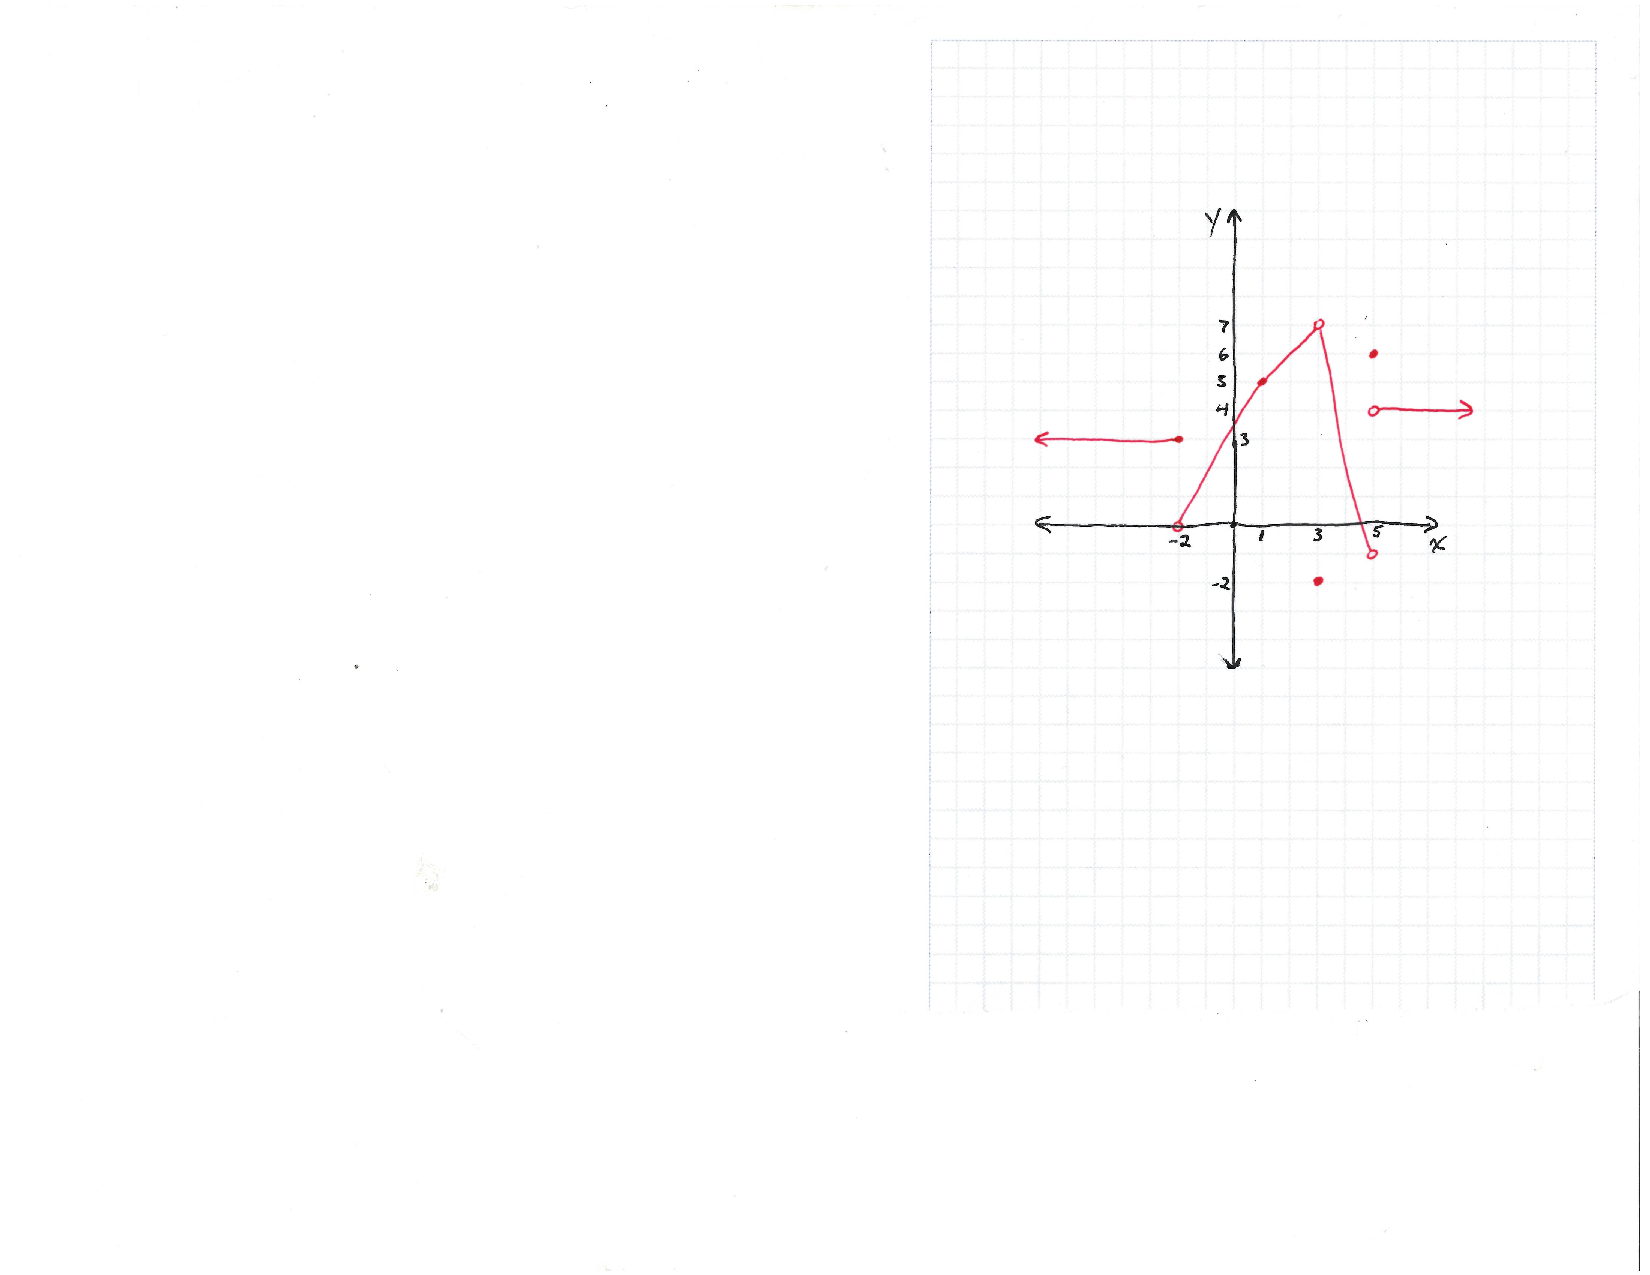
\includegraphics[trim= 450 620 10 0]{Figure3.pdf}
		\end{image}
	\end{freeResponse}
\end{problem}
	










								
				
				
	














\end{document} 


















